\setcounter{section}{4}
\ifanswers
Vi bemærker, at Riemann integrabillitet i alle relevante opgave nedenfor er opfyldt, da alle integrander er kontinuerte på afsluttet begrænset intervaller og dermed Riemann integrable.
\fi
\begin{opg}\hfill \\
	Betragt funktionen $ f\in \text{PCN}_{2\pi} $ givet ved 
	\[ f(x)=x\sin(x), \qquad x\in[-\pi,\pi)
	\]
	og udvidet $2\pi$-periodisk.
	\begin{enumerate}
%		\item Redegør for at $ f $ kan udvides til en lige og stykkevis $ C^1 $ funktion i $ \text{PCN}_{2\pi} $. Beregn $ c_{-1}(f) $,$ c_0(f) $ og $ c_1(f) $.
%		\ifanswers
%		\begin{proof}[Løsning]
%			Det observeres, at $ f(-x)=f(x) $ for alle $ x\in[-\pi,\pi] $, da $ x $ og $ \sin(x) $ hver især er ulige. Definér nu $ \tilde{f}:\R\to\R $ ved $ \tilde{f}(x)=f(x+2\pi k) $ hvis $ k\in\mathbb{Z} $ og $ x+2\pi k\in[-\pi,\pi) $. At $ \tilde{f} $ er veldefineret ses ved, at der for ethvert $ x\in\R $ eksisterer et unikt $ k\in\mathbb{Z} $, således at $ x+2\pi k\in [-\pi,\pi) $. Alternativt, kan man skrive $ \tilde{f}(x)=f\left(x-2\pi\left(\floor{\frac{x-\pi}{2\pi}}+1\right)\right) $.
%			Det gælder trivielt, at $ \tilde{f}(x)=f(x) $ for alle $ x\in[-\pi,\pi) $. Desuden ses det, at $ f(-\pi)=f(\pi)=0 $, hvoraf det følger at $ \tilde{f}(\pi)=f(-\pi)=f(\pi) $. Derfor, er $ \tilde{f} $ en udvidelse af $ f $. Det ses desuden, at $ \tilde{f}(-x)=f(-x+2\pi k)=f(x-2\pi k)=\tilde{f}(x) $, hvor $ k\in\mathbb{Z} $ opfylder at $ -x+2\pi k\in[-\pi,\pi) $, således at $ x-2\pi k\in(-\pi,\pi] $ (hvis $ x-2\pi k=\pi $ så gælder $ f(x-2\pi k)=f(\pi)=f(-\pi)=f(x-2\pi(k+1))=\tilde{f(x)} $). Det gælder tydeligt, at $ \tilde{f(x)}=\tilde{f(x+2\pi)} $ for ethvert $ x\in\R $, så $ \tilde{f} $ er $ 2\pi $-periodisk. Det er derfor nok at tjekke kontinuitet af $ \tilde{f} $ på intervallet $ (-\pi,2\pi) $. Kontinuitet følger direkte af definitionen på $ (-\pi,\pi) $ samt $ (\pi,2\pi) $. Derudover gælder $ \lim\limits_{x\to\pi_-}\tilde{f}(x)=\lim\limits_{x\to\pi_-}f(x)=f(\pi)=0 $, og $ \lim\limits_{x\to\pi_+}\tilde{f}(x)=\lim\limits_{x\to\pi_+}f(x-2\pi)=f(-\pi)=0 $, hvoraf, det følger at $ \tilde{f} $ er kontinuert. Betragt nu $ d_0=-\pi $, $ d_1=\pi $. Da gælder, at restriktionen $ \tilde{f}:[-\pi,\pi]\to\R $ er $ C_1 $, da $ \tilde{f}(x)=f(x) $ for $ x\in[-\pi,\pi] $ samt at $ f'(x)=\sin(x)+x\cos(x) $ er kontinuert på $ (-\pi,\pi) $ og $ \lim\limits_{x\to-\pi_+}f'(x)=-\pi=f'(-\pi) $ og $ \lim\limits_{x\to\pi_-}f'(x)=\pi=f'(\pi) $. Dermed er det vist, at $ f $ kan udvides til en lige stykkevist $ C^1 $ funktion i $ \text{PCN}_{2\pi} $.
%			Koefficienterne $ c_{-1}(f) $,$ c_0(f) $ og $ c_1(f) $ beregnes nu ved \begin{equation*}
%			c_{\pm 1}(f)=\frac{1}{2\pi}\int_{-\pi}^{\pi}f(x)e^{\mp ix} \diff x=\frac{1}{2\pi}\int_{-\pi}^{\pi}x\sin(x)\cos(x) \diff x=\frac{1}{2\pi}\left[\frac{x}{2}\sin^2(x)\right]_{-\pi}^{\pi}-\frac{1}{4\pi}\int_{-\pi}^{\pi}\sin^2(x)\diff x=-\frac{1}{4},
%			\end{equation*}
%			hvor vi har brugt partiel integration, og 
%			$$
%			c_0(f)=\frac{1}{2\pi}\int_{-\pi}^{\pi}x\sin(x)\diff x=\frac{1}{2\pi}\left[x(-\cos(x))\right]_{-\pi}^{\pi}+\frac{1}{2\pi}\int_{-\pi}^{\pi}\cos(x)\diff x=1,
%			$$
%			hvor vi igen har brugt partiel integration.
%		\end{proof}
%		\fi
		\item Beregn $ c_n(f) $ for alle $ n\in\mathbb{Z} $, og opstil Fourierrækken for $ f $. 
		\ifanswers
		\begin{proof}[Løsning]
			Bemærk at $ \sin(x)=\frac{e^{ix}-e^{-ix}}{2i} $. Derfor har vi for $ n\notin\{-1,1\} $\begin{equation*}
			\begin{aligned}
			c_n(f)=\frac{1}{2\pi}\int_{-\pi}^{\pi}f(x)e^{-inx}\diff x=\frac{1}{4\pi i} \left(\int_{-\pi}^{\pi}xe^{-i(n-1)x}\diff x-\int_{-\pi}^{\pi}xe^{-i(n+1)x}\diff x\right)\\
			=\frac{1}{4\pi i} \left(\left[\frac{i}{n-1}xe^{-i(n-1)x}\right]_{-\pi}^{\pi}-\left[\frac{i}{n+1}xe^{-i(n+1)x}\right]_{-\pi}^{\pi}\right)\\
			=\frac{1}{4\pi}\left(\frac{1}{n-1}(-1)^{n-1}2\pi-\frac{1}{n+1}(-1)^{n+1}2\pi\right)\\
			=-\frac{(-1)^n}{n^2-1}.
			\end{aligned}
			\end{equation*}
			For $ n\in\{-1,1\} $ har vi istedet\begin{equation*}
					c_{\pm 1}(f)=\frac{1}{2\pi}\int_{-\pi}^{\pi}f(x)e^{\mp ix} \diff x=\frac{1}{2\pi}\int_{-\pi}^{\pi}x\sin(x)\cos(x) \diff x=\frac{1}{2\pi}\left[\frac{x}{2}\sin^2(x)\right]_{-\pi}^{\pi}-\frac{1}{4\pi}\int_{-\pi}^{\pi}\sin^2(x)\diff x=-\frac{1}{4},
					\end{equation*}
			hvor vi har brugt partiel integration $ \int_{-\pi}^{\pi}\sin^2(x)\diff x=\left[-\cos(x)\sin(x)\right]_{-\pi}^{\pi}+\int_{-\pi}^{\pi}\cos^2(x)\diff x=\int_{-\pi}^{\pi}\cos^2(x)\diff x, $ således at\\ $ \int_{-\pi}^{\pi}\sin^2(x)\diff x=\frac{1}{2}\int_{-\pi}^{\pi}\sin^2(x)+\cos^2(x)\diff x=\pi. $ Dermed ses, at vi har Fourierrækken for $ f $
			$$
			\sum_{n\in \mathbb{Z}}c_n(f)e^{inx}=1-\frac{1}{4}(e^{ix}+e^{-ix})-\sum_{n=2}^{\infty}\frac{(-1)^n}{n^2-1}\left(e^{inx}+e^{-inx}\right).
			$$
		\end{proof}
		\fi
		\item Argumentér for, at $ f $ er stykkevist $ C^1 $, og bevis, at Fourierrækken konvergerer uniformt mod $ f $.
		\ifanswers
		\begin{proof}[Løsning]
			Det ses at $ f $ er kontinuert, da $ f $ er kontinuert på $ (-\pi,\pi) $ samt at $ \lim\limits_{x\to\pi}f(x)=0=f(-\pi)=f(\pi) $.
			Betragt nu indelingen $ d_0=-\pi $, $ d_1=\pi $. Da gælder, at restriktionen $ f:[-\pi,\pi]\to\R $ er $ C_1 $. Dette ses da vi for $ x\in (-\pi,\pi) $ har $ f'(x)=\sin(x)+x\cos(x) $, som er kontinuert på $ (-\pi,\pi) $ samt at $ \lim\limits_{x\to-\pi_+}f'(x)=\pi=f_+'(-\pi) $ og $ \lim\limits_{x\to\pi_-}f'(x)=-\pi=f_-'(\pi) $, hvor $ f_+' $ er den højre afledte og $ f_-' $ er den venstre afledte. Bemærk, at de venstre og højre afledte ovenfor, er lette at finde, da $ f(x)=x\sin(x) $ for alle $ x\in[-\pi,\pi] $, og $ x\sin(x) $ er differentiable overalt.
			
			Det følger da direkte af sætning 5.46, at Fourierrækken konvergerer uniformt mod $ f $.
		\end{proof}
		\fi
		\item Eftervis, at $f$ er lige, og opstil cosinus-rækken for $ f $. Indsæt heri $ x=\pi $ og udled formlen
		$$
		\sum_{n=2}^\infty \frac1{n^2-1}=\frac 34
		$$
		\ifanswers
		\begin{proof}[Løsning]
			At $ f $ er lige ses idet at restriktionen $ f:[-\pi,\pi]\to\R $ er lige, da $ x\mapsto x $ er ulige og $ x\mapsto\sin(x) $ er ulige samt at $ f(\pi)=0=f(-\pi) $).  Siden $ f $ er periodisk per definition, gælder tydeligvis, at $ f\in \text{PCN}_{2\pi} $ er lige. Det findes direkte fra resultatet i b), at $ f(x)=1-\frac{1}{2}\cos(x)-2\sum_{n=2}^{\infty}\frac{(-1)^n}{n^2-1}\cos(nx) $. For $ x=\pi $ finder vi, da $ \cos(n\pi)=(-1)^n $, at $ 0=1+1/2-2\sum_{n=2}^{\infty}\frac{1}{n^2-1} $, hvorfra det følger, at $ \sum_{n=2}^{\infty}\frac{1}{n^2-1}=\frac{3}{4} $.
		\end{proof}
		\fi
		\item Betragt nu funktionen $g\in\text{PCN}_{2\pi}$ som opfylder
		\[
		g(x)=f'(x)=\sin(x)+x\cos(x), \qquad x\in(-\pi,\pi).
		\]
		Find Fourierrækken for $g$
		og vis, at denne konvergerer punktvist mod $ g $. %\textsl{[Bemærk, at $ g $ er den normaliseret stykkevist afledte funktion af $ f $]}.
		\ifanswers
		\begin{proof}[Løsning]
		Da $ f\in \text{PCN}_{2\pi} $ er stykkevist $ C^1 $, følger det af Lemma 5.45, at $ g $ har Fourierkoefficienter $ c_n(g)=inc_n(f) $. Dermed findes Fourierrækken for $ g $ $$
		\sum_{n\in \mathbb{Z}}c_n(g)e^{inx}=\frac{1}{4i}(e^{ix}-e^{-ix})+\sum_{n=2}^{\infty}\frac{(-1)^n}{n-n^{-1}}\frac{1}{i}\left(e^{inx}-e^{-inx}\right).
		$$ 	
		Da $ g\in \text{PCN}_{2\pi} $ er differentiabel fra højre og venstre overalt (siden at $ \sin(x)+x\cos(x) $ er differentiabel overalt) følger det af Sætning 5.40, at Fourierrækken for $ g $ konvergerer punktvist mod $ g $.
		\end{proof}
		\fi
	\end{enumerate}
\end{opg}


\begin{opg}
	Betragt funktionen $ h_0:[-\pi,\pi]\to\C $ givet ved $$
	h_0(x)=\begin{cases}
	e^{ix/2},& -\pi\leq x\leq 0,\\
	ie^{ix/2},& 0<x\leq \pi.
	\end{cases}
	$$
	\begin{enumerate}
		\item Bestem den funktion $ h \in  \text{PCN}_{2\pi} $ der stemmer overens med $ h_0$ undtagen i $ -\pi $, $ 0 $ og $ \pi $.
		\ifanswers
		\begin{proof}[Løsning]
			Betragt den periodiske udvidelse, $ h $, af $ \tilde{h}:[-\pi,\pi)\to\C $ givet ved $$ \tilde{h}(x)=\begin{cases}
			-\frac{1+i}{2},& x=-\pi,\\
			\frac{1+i}{2},& x=0,\\
			h_0(x),&x\in(-\pi,\pi)\setminus\{0\}.
			\end{cases} $$
			Da opfylder $ h $ betingelserne i opgaven.
		\end{proof}
		\fi
		\item Vis at $ c_n(h)=\dfrac{1+i}{\pi(n-1/2)} $ for alle ulige $ n $, og at $ c_n(h)=0 $ for alle lige $ n $.
		\ifanswers
		\begin{proof}[Løsning]
			Vi har $$
			c_n(h)=\frac{1}{2\pi}\left(\int_{-\pi}^{0}e^{ix/2}e^{-inx} \diff x+i\int_{0}^{\pi}e^{ix/2}e^{-inx} \diff x\right)=\frac{1}{2\pi}\left(\frac{(1-e^{i\pi(n-1/2)})}{-i(n-1/2)}+i\frac{(e^{-i\pi(n-1/2)}-1)}{-i(n-1/2)}\right).
			$$
			Det følger ved brug af $ e^{i\pi}=-1 $ samt $ e^{\pm i\pi/2}=\pm i $ at$$
			c_n(h)=-\frac{1}{i2\pi(n-1/2)}(1-i+(-1)^ni+i(-1^n)i)=\frac{1}{2\pi(n-1/2)}(1+i)(1-(-1)^n).
			$$
			Heraf ses let at $ c_n(h)=\frac{1+i}{\pi(n-1/2)} $ for $ n $ ulige, og $c_n(h)=0  $ for $ n $ lige.
		\end{proof}
		\fi
		\item Vis, at $$ \sum_{\begin{array}{c}\scriptstyle n=-\infty\\\scriptstyle n\text{ ulige}\end{array}}^\infty \dfrac{1+i}{\pi(n-1/2)}e^{inx}=h(x) $$ punktvist for alle $ x\in\mR$. Afgør om konvergensen er uniform.
		\ifanswers
		\begin{proof}[Løsning]
			Da $ h\in \text{PCN}_{2\pi} $ er differentiabel fra højre og venstre overalt (siden at $ e^{ix/2} $ og $ ie^{ix/2} $ hver især er differentiable overalt), følger det af sætning 5.40, at Fourierrækken for $ h $ konvergerer punktvist mod $ h $. Altså har vi $ \sum_{\substack{n=-\infty\\
					n\text{ ulige}}}^{\infty} \frac{1+i}{\pi(n-1/2)}e^{inx}=h(x) $ for alle $ x\in\R $ og dermed specielt for alle $ x\in[-\pi,\pi] $ som ønsket.\\
			Bemærk, hvis konvergensen var uniform ville grænsen, $ h $, nødvendigvis være kontinuert per Sætning 3.13 hvor vi identificerer afsnitssummerne med en uniform konvergent funktionsfølge. Men $ h $ er ikke kontinuert, hvorfor konvergensen ikke er uniform. 
		\end{proof}
		\fi
		\item Illustrer $ h $ sammen med afsnitssummerne $ \tau_1$, $ \tau_3 $ og $ \tau_5 $ for Fourierr\ae{}kken, opfattet som kurver i den komplekse plan.
		\begin{proof}[Løsning]\hfill
			\ifanswers \begin{center}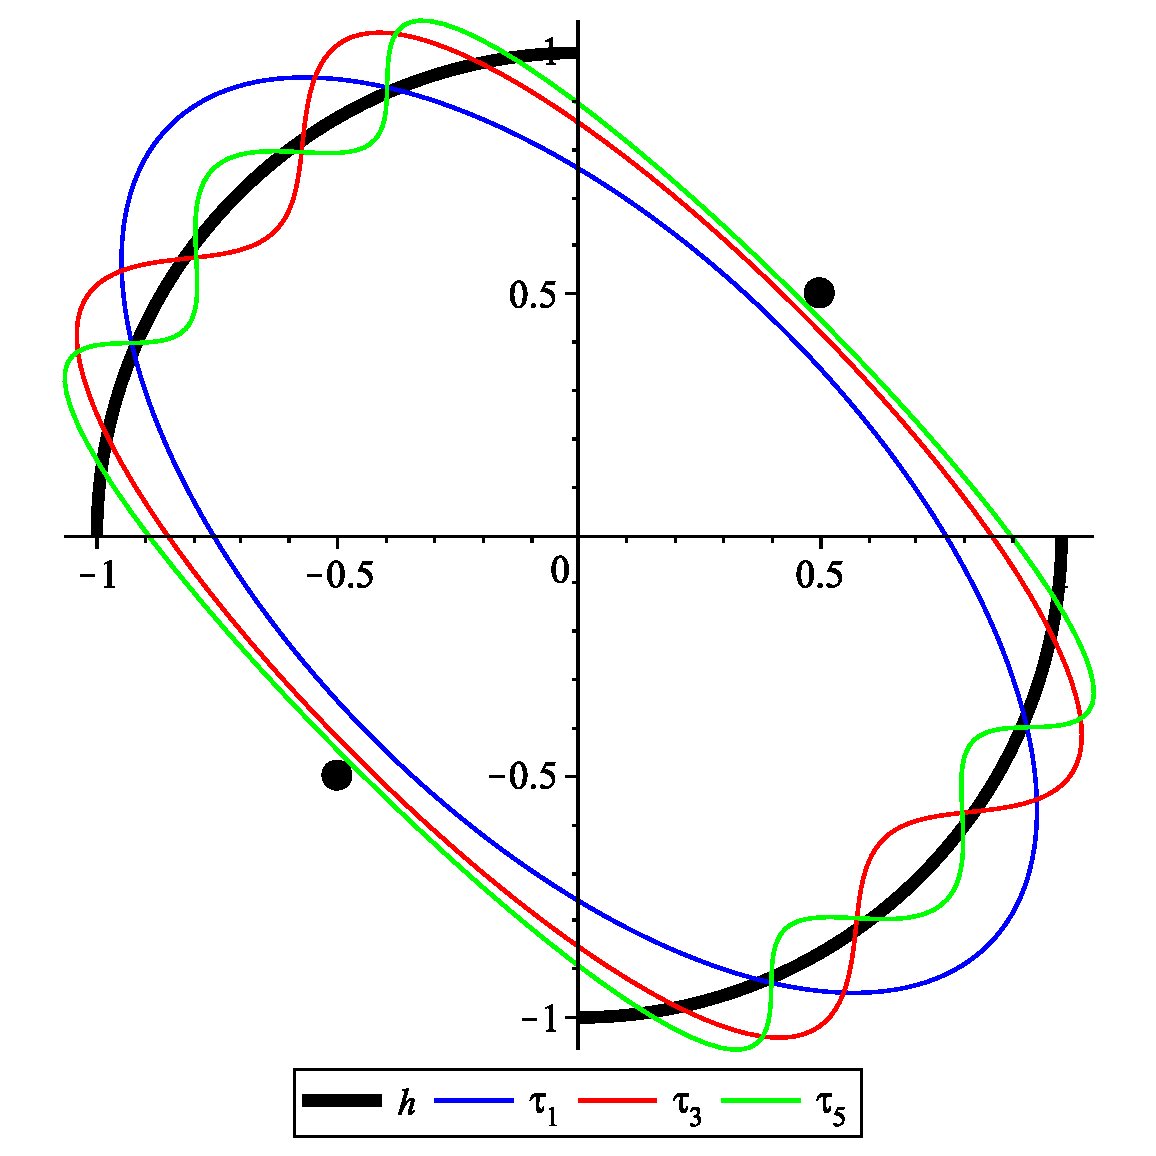
\includegraphics[width=8cm]{for4bedre}\end{center}\fi
		\end{proof}
	\end{enumerate}
\end{opg}
\begin{opg}\hfill \\
	I denne opgave ser vi på to metrikker på $ \R $, nemlig den diskrete metrik $ d_\text{disk} $ og den sædvanlige metrik $ d(x,y)=\abs{y-x} $.
	Lad $ A=(\R,d_{\text{disk}}) $ og $ B=(\R,d) $ være de to metriske rum der begge har $ \R $ som underliggende mængde, men er udstyret med de to forskellige metrikker som anført.
	\begin{enumerate}
		\item Vis at enhver funktion $ f:A\to B $ er kontinuert. \textsl{[Hvis man benytter Eksempel 6.51 skal det forklares hvorfor alle delmængder er åbne i $ A $]}
		\ifanswers
		\begin{proof}[Løsning]
			Bemærk, at i et diskret metrisk rum, $ M $, gælder, at $ K(x,1/2)=\{x\} $ for alle $ x\in M $. Dermed gælder for enhver delmængde $ N\subset M $, at $ x\in N $ er et indre punkt, da $ K(x,1/2)=\{x\}\subset N $. Så $ N $ er åben i $ M $. Det følger nu af Sætning 6.50, at enhver funktion, $ f:A\to B $, er kontinuert da $ f^{-1}(G) $ er åben i $ A $ for enhver (åben) delmængde $ G\subset B $.
		\end{proof}
		\fi
		\item Vis at en funktion $ f:B\to A $ er kontinuert hvis og kun hvis den er konstant, altså hvis $ f(x)=c $ for et fast $ c\in \R $ og for alle $ x\in\R  $.
		\textsl{[Vink: Brug supremumsegenskaben for $ \R $ direkte eller indirekte]}
		\ifanswers
		\begin{proof}[Løsning]
			Bemærk først, at hvis en ikke-tom delmængde $ U\subset B $ er åben og afsluttet, så er $ U=\R $. For at se dette, lad $ x_0\in U $, og betragt mængden $ S=\{r>0: [x_0-r,x_0+r]\subset U\} $, som er ikke-tom da $ U $ er åben. Antag for modstrid, at $ S $ er begrænset. Lad da $ R=\sup(S) $ (hvor vi har brugt supremumsegenskaben for de reelle tal) og lad $ \seq {r^\pm} $ være en følge i $ S $ der konvergerer mod $ \pm R $. Siden $ U $ er afsluttet, gælder det per Lemma 6.58, at $ x_0\pm R=\lim\limits_{n\to\infty}(x_0+r^\pm_n)\in U $, hvorfor der eksisterer $ \delta_\pm>0 $ således at $ (x_0\pm R-\delta_\pm,x_0\pm R+\delta_\pm)\subset U $, hvilket er modstrid med definitionen af $ R $ for mindst et af fortegnene $ \pm $. Vi konkluderer at $ S $ er ubegrænset, hvoraf det følger, at $ U=\R $.\\
			Lad $ f:B\to A $ være kontinuert, og lad $ c\in f(B) $. Som argumenteret i a), er enhver delmængde af $ A $ åben. Betragt nu den ikke-tomme åbne (pga. kontinuitet og Sætning 6.50) mængde $ O=f^{-1}\left(\{c\}\right) $. Bemærk, at siden alle mængder er åbne i et diskret metrisk rum, er alle mængder også afsluttede per Sætning 6.55. Det gælder dermed klart at $ \{c\} $ er afsluttet i $ A $, hvorfor $ O $ også er afsluttet i $ B $ ved kontinuitet af $ f $ (opgave 9.1.b) på ugeseddel 9). Det konkluderes at $ O $ er ikke-tom, åben og afsluttet i $ B $, hvorfor $ O=\R $, og det følger at $ f(x)=c $ for alle $ x\in\R $. Modsat gælder der trivielt, hvis $ f $ er konstant, at $ f(x_n)\to c=f(x) $ for $ x_n\to x $ når $ n\to\infty $. Det følger da af sætning 6.37, at $ f $ er kontinuert.
			
			
%			betragt derfor de to (åbne) delmængder af $ A $, $ O_1=\{x\in A\vert x<c\} $ og $ O_2=\{x\in A\vert x\geq c\} $. Da gælder at $ f^{-1}(O_1) $ og $ f^{-1}(O_2)$ er disjunkte og åbne, samt at $ f^{-1}(O_1)\cup f^{-1}(O_2)=f^{-1}(O_1\cup O_2)=\R $. Dette er kun muligt, hvis $ f^{-1}(O_1)=\emptyset $ eller $ f^{-1}(O_1)=\emptyset $. Men da $ f^{-1}(O_2)\neq \emptyset $ konkludere vi at $ f^{-1}(O_2)=\R $ hvoraf det følger, at $ f(x)\geq c $ for alle $ x\in \R $, på den anden side kan vi udfører samme argument med $ \tilde{O}_1=\{x\in A\vert x>c\} $ og $ \tilde{O}_2=\{x\in A\vert x\leq c\} $ hvoraf, det følger at $ f(x)\leq c $ for alle $ x\in \R $. Dermed er det vist, at $ f $ er konstant. 
		\end{proof}
		\fi
	\end{enumerate}
\end{opg}